% Architecture diagram for NL-SRE-English
% Requires: \usepackage{tikz}
% Usage: % Architecture diagram for NL-SRE-English
% Requires: \usepackage{tikz}
% Usage: % Architecture diagram for NL-SRE-English
% Requires: \usepackage{tikz}
% Usage: % Architecture diagram for NL-SRE-English
% Requires: \usepackage{tikz}
% Usage: \input{figures/fig_architecture.tex}

\begin{figure}[htbp]
\centering
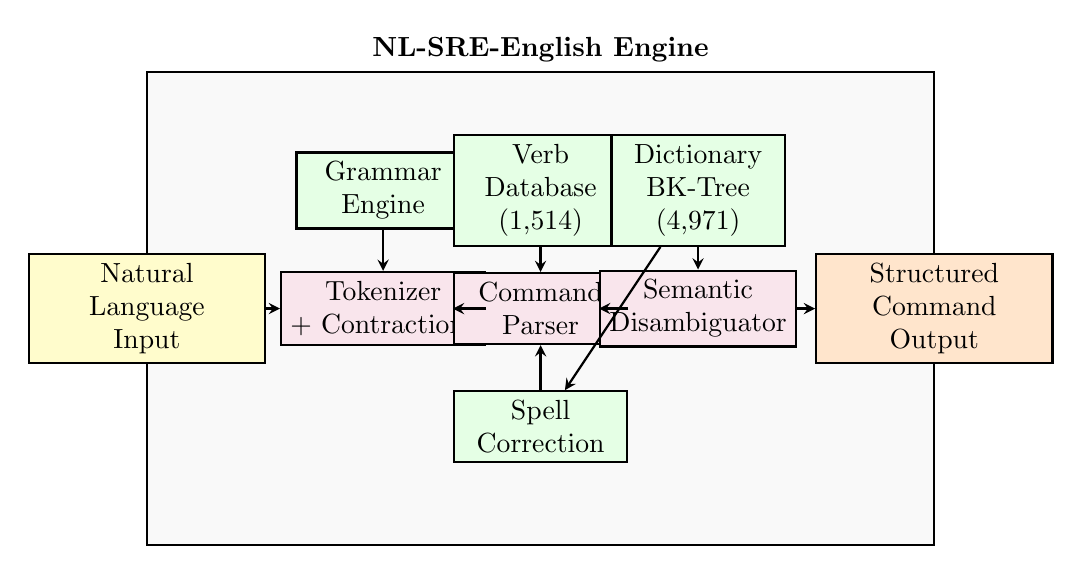
\begin{tikzpicture}[
    node distance=1.5cm,
    box/.style={rectangle, draw=black, thick, minimum width=3cm, minimum height=1cm, align=center, fill=blue!10},
    smallbox/.style={rectangle, draw=black, thick, minimum width=2.2cm, minimum height=0.8cm, align=center, fill=green!10},
    arrow/.style={->, thick, >=stealth}
]

% Main container
\node[box, minimum width=10cm, minimum height=6cm, fill=gray!5] (main) at (0,0) {};
\node[above] at (main.north) {\textbf{NL-SRE-English Engine}};

% Input
\node[box, fill=yellow!20] (input) at (-5, 0) {Natural\\Language\\Input};

% Output
\node[box, fill=orange!20] (output) at (5, 0) {Structured\\Command\\Output};

% Internal components
\node[smallbox] (grammar) at (-2, 1.5) {Grammar\\Engine};
\node[smallbox] (verbs) at (0, 1.5) {Verb\\Database\\(1,514)};
\node[smallbox] (dict) at (2, 1.5) {Dictionary\\BK-Tree\\(4,971)};

\node[smallbox, fill=purple!10] (tokenizer) at (-2, 0) {Tokenizer\\+ Contractions};
\node[smallbox, fill=purple!10] (parser) at (0, 0) {Command\\Parser};
\node[smallbox, fill=purple!10] (disamb) at (2, 0) {Semantic\\Disambiguator};

\node[smallbox] (spell) at (0, -1.5) {Spell\\Correction};

% Arrows
\draw[arrow] (input) -- (tokenizer);
\draw[arrow] (tokenizer) -- (parser);
\draw[arrow] (parser) -- (disamb);
\draw[arrow] (disamb) -- (output);

\draw[arrow] (grammar) -- (tokenizer);
\draw[arrow] (verbs) -- (parser);
\draw[arrow] (dict) -- (disamb);
\draw[arrow] (spell) -- (parser);
\draw[arrow] (dict) -- (spell);

\end{tikzpicture}
\caption{NL-SRE-English system architecture showing the processing pipeline from natural language input to structured command output.}
\label{fig:architecture}
\end{figure}


\begin{figure}[htbp]
\centering
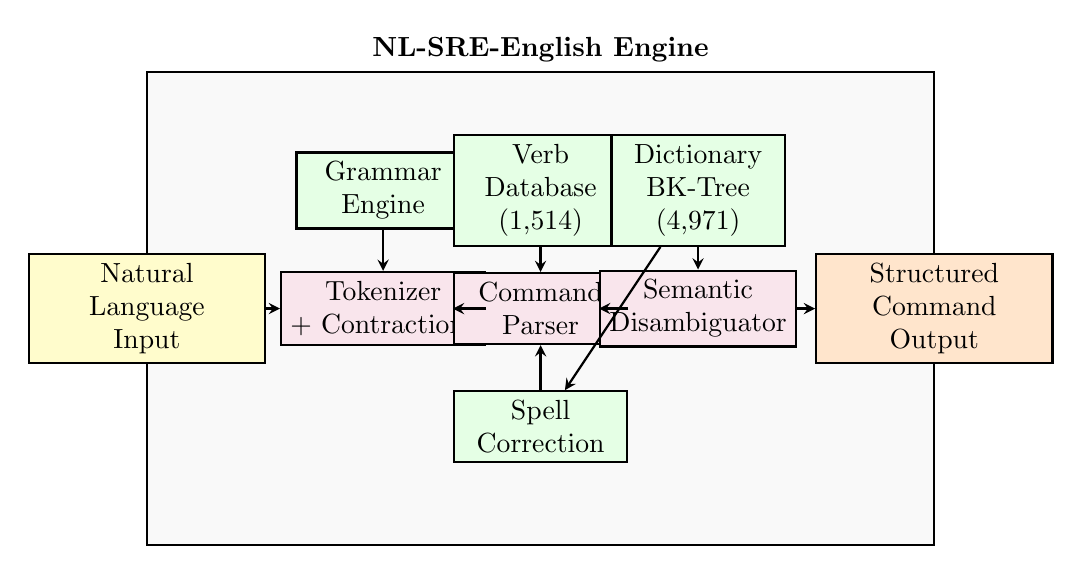
\begin{tikzpicture}[
    node distance=1.5cm,
    box/.style={rectangle, draw=black, thick, minimum width=3cm, minimum height=1cm, align=center, fill=blue!10},
    smallbox/.style={rectangle, draw=black, thick, minimum width=2.2cm, minimum height=0.8cm, align=center, fill=green!10},
    arrow/.style={->, thick, >=stealth}
]

% Main container
\node[box, minimum width=10cm, minimum height=6cm, fill=gray!5] (main) at (0,0) {};
\node[above] at (main.north) {\textbf{NL-SRE-English Engine}};

% Input
\node[box, fill=yellow!20] (input) at (-5, 0) {Natural\\Language\\Input};

% Output
\node[box, fill=orange!20] (output) at (5, 0) {Structured\\Command\\Output};

% Internal components
\node[smallbox] (grammar) at (-2, 1.5) {Grammar\\Engine};
\node[smallbox] (verbs) at (0, 1.5) {Verb\\Database\\(1,514)};
\node[smallbox] (dict) at (2, 1.5) {Dictionary\\BK-Tree\\(4,971)};

\node[smallbox, fill=purple!10] (tokenizer) at (-2, 0) {Tokenizer\\+ Contractions};
\node[smallbox, fill=purple!10] (parser) at (0, 0) {Command\\Parser};
\node[smallbox, fill=purple!10] (disamb) at (2, 0) {Semantic\\Disambiguator};

\node[smallbox] (spell) at (0, -1.5) {Spell\\Correction};

% Arrows
\draw[arrow] (input) -- (tokenizer);
\draw[arrow] (tokenizer) -- (parser);
\draw[arrow] (parser) -- (disamb);
\draw[arrow] (disamb) -- (output);

\draw[arrow] (grammar) -- (tokenizer);
\draw[arrow] (verbs) -- (parser);
\draw[arrow] (dict) -- (disamb);
\draw[arrow] (spell) -- (parser);
\draw[arrow] (dict) -- (spell);

\end{tikzpicture}
\caption{NL-SRE-English system architecture showing the processing pipeline from natural language input to structured command output.}
\label{fig:architecture}
\end{figure}


\begin{figure}[htbp]
\centering
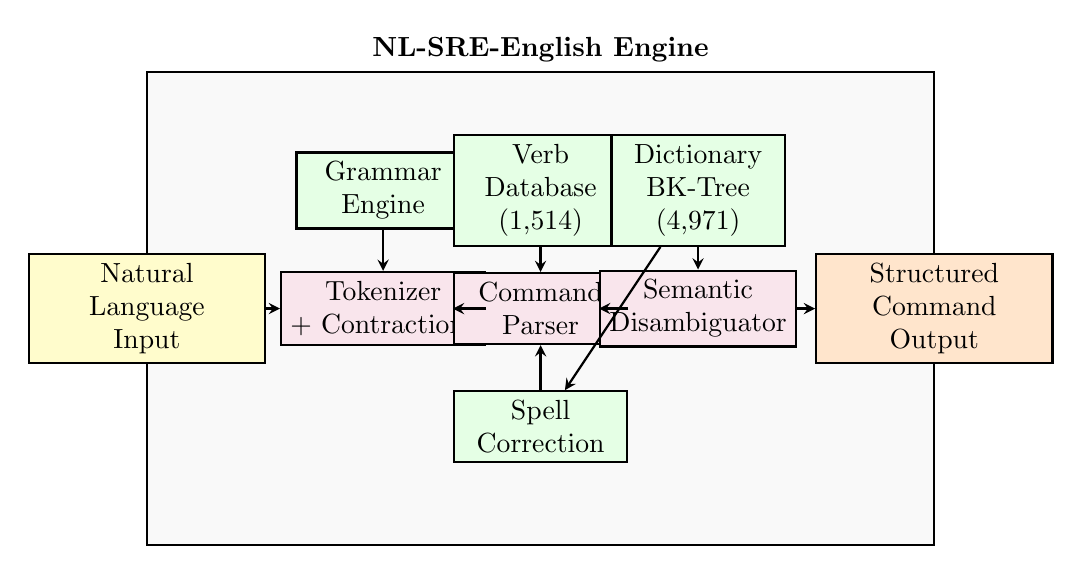
\begin{tikzpicture}[
    node distance=1.5cm,
    box/.style={rectangle, draw=black, thick, minimum width=3cm, minimum height=1cm, align=center, fill=blue!10},
    smallbox/.style={rectangle, draw=black, thick, minimum width=2.2cm, minimum height=0.8cm, align=center, fill=green!10},
    arrow/.style={->, thick, >=stealth}
]

% Main container
\node[box, minimum width=10cm, minimum height=6cm, fill=gray!5] (main) at (0,0) {};
\node[above] at (main.north) {\textbf{NL-SRE-English Engine}};

% Input
\node[box, fill=yellow!20] (input) at (-5, 0) {Natural\\Language\\Input};

% Output
\node[box, fill=orange!20] (output) at (5, 0) {Structured\\Command\\Output};

% Internal components
\node[smallbox] (grammar) at (-2, 1.5) {Grammar\\Engine};
\node[smallbox] (verbs) at (0, 1.5) {Verb\\Database\\(1,514)};
\node[smallbox] (dict) at (2, 1.5) {Dictionary\\BK-Tree\\(4,971)};

\node[smallbox, fill=purple!10] (tokenizer) at (-2, 0) {Tokenizer\\+ Contractions};
\node[smallbox, fill=purple!10] (parser) at (0, 0) {Command\\Parser};
\node[smallbox, fill=purple!10] (disamb) at (2, 0) {Semantic\\Disambiguator};

\node[smallbox] (spell) at (0, -1.5) {Spell\\Correction};

% Arrows
\draw[arrow] (input) -- (tokenizer);
\draw[arrow] (tokenizer) -- (parser);
\draw[arrow] (parser) -- (disamb);
\draw[arrow] (disamb) -- (output);

\draw[arrow] (grammar) -- (tokenizer);
\draw[arrow] (verbs) -- (parser);
\draw[arrow] (dict) -- (disamb);
\draw[arrow] (spell) -- (parser);
\draw[arrow] (dict) -- (spell);

\end{tikzpicture}
\caption{NL-SRE-English system architecture showing the processing pipeline from natural language input to structured command output.}
\label{fig:architecture}
\end{figure}


\begin{figure}[htbp]
\centering
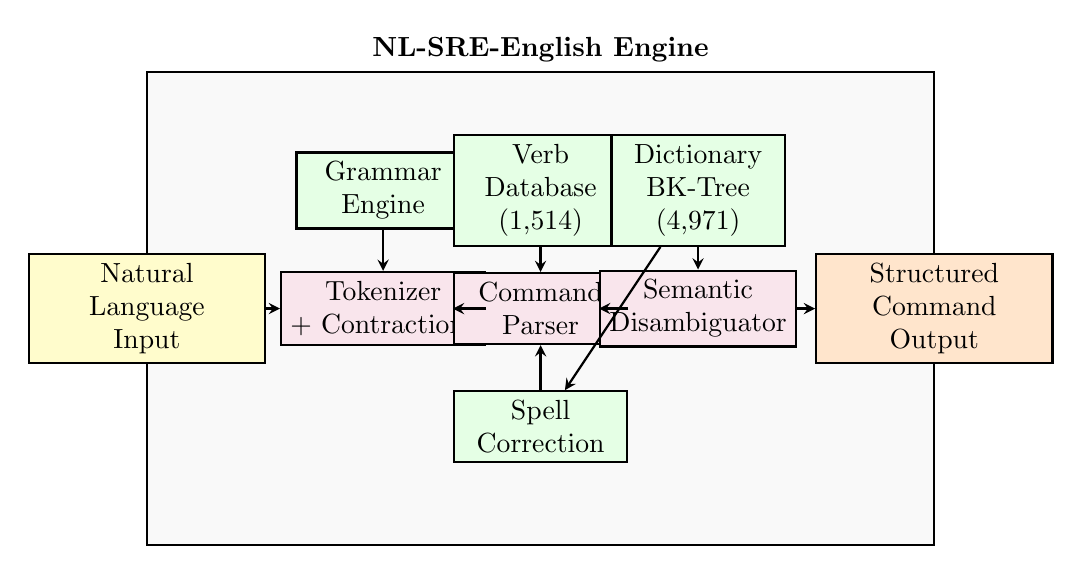
\begin{tikzpicture}[
    node distance=1.5cm,
    box/.style={rectangle, draw=black, thick, minimum width=3cm, minimum height=1cm, align=center, fill=blue!10},
    smallbox/.style={rectangle, draw=black, thick, minimum width=2.2cm, minimum height=0.8cm, align=center, fill=green!10},
    arrow/.style={->, thick, >=stealth}
]

% Main container
\node[box, minimum width=10cm, minimum height=6cm, fill=gray!5] (main) at (0,0) {};
\node[above] at (main.north) {\textbf{NL-SRE-English Engine}};

% Input
\node[box, fill=yellow!20] (input) at (-5, 0) {Natural\\Language\\Input};

% Output
\node[box, fill=orange!20] (output) at (5, 0) {Structured\\Command\\Output};

% Internal components
\node[smallbox] (grammar) at (-2, 1.5) {Grammar\\Engine};
\node[smallbox] (verbs) at (0, 1.5) {Verb\\Database\\(1,514)};
\node[smallbox] (dict) at (2, 1.5) {Dictionary\\BK-Tree\\(4,971)};

\node[smallbox, fill=purple!10] (tokenizer) at (-2, 0) {Tokenizer\\+ Contractions};
\node[smallbox, fill=purple!10] (parser) at (0, 0) {Command\\Parser};
\node[smallbox, fill=purple!10] (disamb) at (2, 0) {Semantic\\Disambiguator};

\node[smallbox] (spell) at (0, -1.5) {Spell\\Correction};

% Arrows
\draw[arrow] (input) -- (tokenizer);
\draw[arrow] (tokenizer) -- (parser);
\draw[arrow] (parser) -- (disamb);
\draw[arrow] (disamb) -- (output);

\draw[arrow] (grammar) -- (tokenizer);
\draw[arrow] (verbs) -- (parser);
\draw[arrow] (dict) -- (disamb);
\draw[arrow] (spell) -- (parser);
\draw[arrow] (dict) -- (spell);

\end{tikzpicture}
\caption{NL-SRE-English system architecture showing the processing pipeline from natural language input to structured command output.}
\label{fig:architecture}
\end{figure}
